\chapter{Conclusions and Future Work}
\label{chp-con}

In this dissertation, we aim to strengthen dependability of cloud-scale
distributed systems by addressing two new types of bugs in cloud systems,
distributed concurrency bugs (DC bugs) and scalability bugs. We have performed
bug studied to gain insights about the nature of these bugs, and we have also
advanced state of the art of system testing. This chapter concludes this
dissertation work and discuss future work in combating DC bugs and scalability
bugs.

\section{Conclusion}

\subsection{Distributed Concurrency Bugs}

The first problem we focus in this dissertation is DC bugs. We have conducted
in-depth study and created the largest and most comprehensive of DC bugs named
\taxdc. We categorize DC bugs in three dimensions. The first dimension is
triggering which is conditions that makes bugs happens. We studied timing
conditions and found four main timing patterns: order violation, atomicity
violation, fault timing, and reboot timing. We also studied input conditions
that are ingredients for bugs to surface. We found that most DC bugs will
surface only systems execute multiple protocols, and more than 50\% of bugs
surface in recovery protocols (\ie, the bugs surface only when there are
hardware failures).

The second dimension that we studied is errors and failures. We studied the
first errors that happen immediately after the bugs are triggered. We see half
of the bugs have local errors that is we can see the errors by observing only
triggering node, but half of them have global errors that require us to observe
the whole systems to notice the errors. Moreover, we looked into failure
symptom induced by DC bugs and found that the bugs can lead to severe failures
like system downtime, operation failures, data loss/corruption/inconsistencies,
and performance degradation.

Lastly, the third dimension that we studied is fixes that are how developers fix
the DC bugs. We saw two main strategies to fix the bugs that are fixing the
timing and fixing the handling. For timing fixes, developers can do it globally or
locally (global synchronization or local synchronization). For handling fixes,
developers change the logic of message handling or fault handling such that the
systems still behave correctly.

Other than the bug study, we have introduced semantic-aware model checking
(SAMC) that is a white-box approach to model check the systems. SAMC prunes out
some executions because it knows that those executions are redundant with
previous executions it already tested by using semantic knowledge of target
systems. We show a strong case that SAMC can elegantly address
state-space-explosion problem. We have introduced four novel semantic-aware
reduction policies, and built \sampro\ and integrated it to three systems
including Hadoop MapReduce, Cassandra and ZooKeeper. On average, SAMC can find
bugs 49x faster than other states of the art.

\subsection{Scalability Bugs}

The second problem we focus in this dissertation is scalability bugs.
Scalability bugs are bugs that specific to cloud systems and we found there is
not much attention paid on them. We observed that scalability bugs are scale
dependent and only surface at extreme scale (\eg, hundreds of nodes). We noticed
that although the systems are designed to be scalable, but actual
implementations can introduces the bugs. We also saw that not all developers can
afford large clusters to check scalability of their code, and make bugs linger
until the systems are deployed on large scale.

Our observations highlight the need for scale checking that check the
implementation of the systems. Hence, we have introduced \sck, a scale-checking
methodology to allow developers colocate hundreds nodes on a single machine to
check their systems. We introduced four techniques to mitigate resource
contentions issue (\ie, CPU, memory, and threads) regarding to colocating
several nodes in one machine. We adopted \sck to three systems including
Cassandra, Riak, and Voldemort, and were able to reproduce six old scalability
bugs with high accuracy.

\if 0
\section{Future Work}

\subsection{Automated Semantic Extracting for SAMC}
\label{sec-autosamc}

So far SAMC requires developers to manually extract semantic knowledge for dmck
and write the corresponding reduction policies manually. This manual step is
based on high-level human understanding of the code, which can be error-prone.
The developers can also introduce human errors when writing reduction policies
and breaks soundness. Thus, when the current SAMC does not find bugs, it does
not imply systems are bug-free; some bugs might be accidentally missed by wrong
policies. Currently, there is no way to verify that the semantics used for
pruning out executions is correct.

To address these limitations, we propose ``\textit{automated semantic extracting
tool}'' (ASE), a tool that automatically extracts useful semantic knowledge to
build reduction policies. To achieve this goal, we will create an advanced
source code analysis tool that adopts symbolic execution. Symbolic execution
generates constraints at condition statements that define predicate values
leading to true and false conditions. The collection of condition constraints
leading to a specific path in the code is called a path constraint. Others have
used symbolic execution to target system problems
\cite{Bucur+14-SymbolicExecution}, but ASE is different. For instance, we want
to build path constraints that lead to state updates but whose states stay the
same regardless of the reordering (\eg, discard, increment, and constant
patterns) or path constraints that lead to state-update independence. Each path
constraint can be a function of the local state of each node and the messages
the node receives. Generating such a path constraint will require a symbolic
execution tool with additional new supports.

Another benefit of ASE is it allows complex processing patterns to be leveraged
in reduction. So far, we have introduced only simple patterns (\eg, discard,
increment, and constant patterns), because these patterns are easy to be
manually extracted with small chance of human errors. But if ASE is built, it
allows us to introduce more sophisticated patterns and policies without many
burdens on developers. We believe that ASE is a key factor to make SAMC adopted
widely.

\subsection{Automatic Scalability Checking Tool}

\sck that we have introduced is a methodology to assist developers to
scale-check the systems, however, it requires a great amount of efforts to
integrate to development processes.  Developers needs to modify their codebase
to adopt PIL, SPC, GEDA, and MFR as we have shown in Table \ref{tab-loc}. \sck
also requires high-level of code understanding from developers to point out
PIL-safe functions. We consider this as a great cost that hinders \sck to be
adopted, so in this section we present the plausibility to make the whole
process become automatic.



\def \fgw {0.85in}


\begin{figure*}[t]

\centerline{
%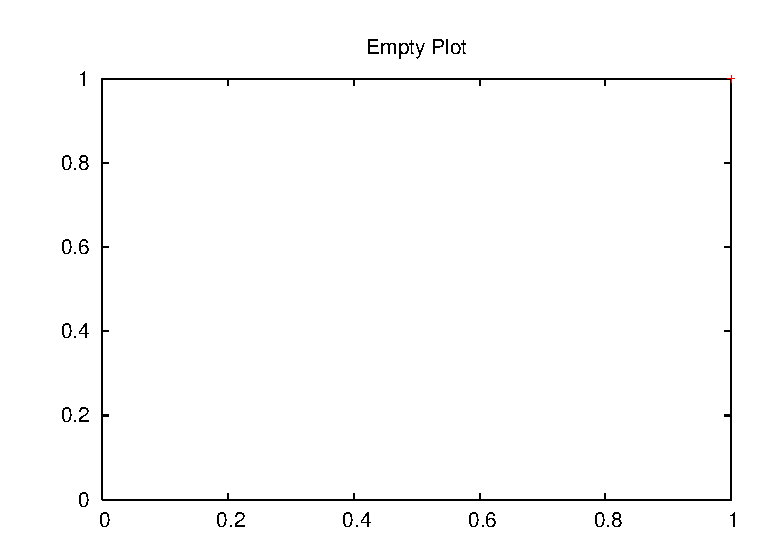
\includegraphics[height=\fgw]{F/empty.eps}
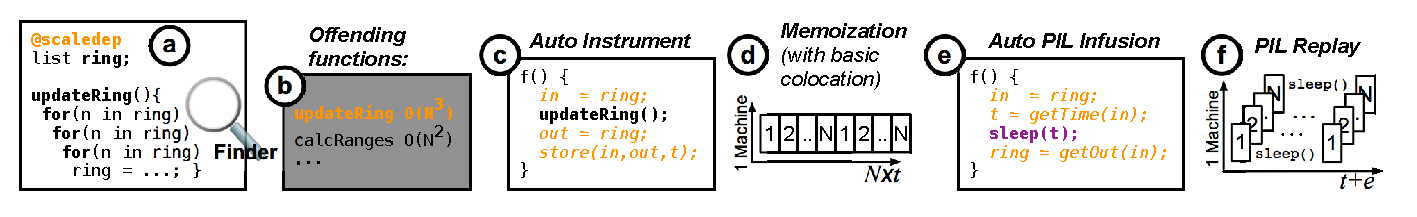
\includegraphics[height=\fgw]{F/ill/sck1-hotos.eps}
}

\mycaption{fig-arch}{The proposed flow of an automated scale-check process}{The 
figure is described in Section \sec\ref{sec-future}.}



\end{figure*}



Figure \ref{fig-arch} depicts the whole scale-check process that we propose as
we explain below:
%
\begin{enumerate}[label=(\alph*)]

\item First, developers annotate data structures that are scale dependent.
%
\item The PIL-safe and offending function finder (a program analysis) will find
loops that are scale dependent (that iterate on the scale-dependent data
structures). This program analysis will provide reports of offending functions
along with the paths (if-else branches) that would exercise them, so that the
developers can set up the corresponding test workloads (\eg, rebalancing,
decommissioning).
%  and the protocols to be tested;
%
\item The finder also automatically inserts input/output/time recording around
the offending functions.
%
\item The target protocols are executed for pre-memoization, which takes time
but only a one-time overhead.
%
\item The deterministic replayer automatically replaces the expensive functions
with \ts{sleep(t)} and copy the output from the memoization database.
%
\item Finally, the fast and accurate PIL-infused replay can begin, and if
needed, the developers can add more logs to debug the code at step e and replay
again.

\end{enumerate}

From this proposal, the integration of \sck is nearly automated. The only step
developers need to do is step a) (\ie, annotating scale-dependent data
structures) which we believe this task is not burdensome, and the rest will be
handled by the program analysis tool (step b) and code transformation tool (step
c and d).
\fi

\section{Future Work}
\label{sec-less}

We now discuss our research impact and future research revenues in combating DC
bugs and scalability bugs. Regarding DC-bug combating, although many high-level
directions can be adopted from work on LC bugs, there are many interesting
challenges and opportunities unique to DC bugs. For scalability bugs, our pilot
work just targets a subset of scalability bugs, there are many classes of
scalability bugs that we have not touched yet.

\subsection{Distributed Concurrency Bugs}
% ===========================================================
\subsubsection{Fault Paths and Multi-Protocol Interactions}
\label{less-fault}

Individual protocols tend to be robust in general.  Only 18 DC bugs
occur in {\em individual} protocols {\em without} any input 
fault condition; only
8 of them are in foreground protocols.  On the other hand, a large
majority of DC bugs happen due to concurrent executions of multiple
protocols and/or different fault timings (Finding {\bf \#2}).
%
This has a tremendous implication to input testing: {\em all types of
  verification, testing, and analysis approaches must consider fault
  injections and multiple protocols as input conditions.}
%
Although recent work has paid attention to this
\cite{Gunawi+11-FateDestini, Joshi+11-PreFail, 
Yuan+14-SimpleTesting}, we emphasize
that all forms of faults (\sec\ref{met-pres}) must be exercised.


% ======================================================
\subsubsection{Distributed Systems Model Checkers}
\label{less-dmck}

Assuming the necessary input conditions are exercised, the next
question is: can we test different event re-orderings to hit the
triggering timing (\sec\ref{trig-time})?  This is the job of
distributed system model checkers (dmck), which are gaining popularity
recently \cite{Guo+11-Demeter, 
Killian+07-LifeDeathMaceMC,
  Simsa+10-Dbug,
  Yang+09-Modist}.  Dmck works by intercepting distributed events and
permuting their ordering.  The more events included, the more
scalability issues will arise due to state-space explosion.
%
To date, {\em no dmck completely controls the timings of
  \underline{all} necessary events} that might contribute to the
triggering timing (Finding {\bf \#1}).  MaceMC
\cite{Killian+07-LifeDeathMaceMC} only reorders messages and network
disconnections.  MoDist \cite{Guo+11-Demeter} exercises timeouts and
Demeter \cite{Guo+11-Demeter} intercepts messages and local
computation but they do not explore different timing of multiple
crashes and reboots. Also, none of the above include storage faults
or timing issues \cite{Hao+16-TailAtStore}.
%
Therefore, continued research on scalable exploration algorithms is
needed, specifically 
% to reduce the state-space explosion 
when {\em all} the necessary events need to be controlled.
This could be helped by DC bugs' triggering scope characteristics
(Finding {\bf \#3}), just like that in
LC model checkers \cite{madanpldi07}.


% ======================================================
\subsubsection{Domain-Specific Specifications}
\label{less-spec}

Now, assuming the necessary events are controlled, the next question
is: do we have the specification to judge the manifestation of a bug?  
This is a plague for many tools. For example,
Demeter does not find new bugs \cite{Guo+11-Demeter}.
Conversations with the authors suggest that their target systems do
not deploy detailed specifications, and thus some bugs are left
uncaught.  Deploying generic ``textbook'' specifications (\eg, ``only
one leader exists'') does not help as they could lead to false
positives (\eg, ZooKeeper allows two leaders at a single point in
time).  Many research papers on specifications only deploy few of them
\cite{Gunawi+11-FateDestini, Liu+08-D3S, Reynolds+06-Pip}.
Developers also
bemoan the hard-to-debug fail-silent problems \mr{3634} and
prefer to see easier-to-debug fail-stop bugs.  
%

On the positive side, \pctErrExp\ of DC bugs lead to
explicit first errors (Finding {\bf \#4}), implying that sanity checks
already in software can be harnessed as 
specifications
(more in \sec\ref{less-det}). On the other side, compared to
single-machine systems, distributed systems are much more capable
of masking errors. Therefore, these error
specifications have to be used with caution to avoid false 
positives. Furthermore, 
\pctErrImp\ of DC bugs lead to silent first errors (Finding {\bf \#4}).
Many of them proceed to ``silent failures'', such as data loss,
node hangs, etc. Even if they become explicit
errors later, these explicit errors could be far away from the 
initial triggering conditions (\eg, Figure \ref{fig-paxos}).
In short, {\em no matter how sophisticated the tools are, they are
  ineffective without accurate specifications}.
%
This motivates the creation or inference of local specifications
that can show early errors or symptoms of DC bugs.


% ======================================================
\subsubsection{Bug Detection Tools}
\label{less-det}

%We emphasize that the state of the art solutions for dc bugs fall into
%three camps: testing and model checking \cite{x}, verifiable
%distributed system frameworks \cite{x}, postmortem monitoring and
%debugging \cite{x}.  

We now discuss bug detection tools, which are
unfortunately rare for DC bugs, although very popular for
LC bugs
%
\cite{pacer,
  flanagan09fasttrack, 
  satish.pldi14, 
  avio.asplos06, 
  madanpldi07,
  savage97eraser}.
%
Bug detection tools look for bugs that match specific patterns.  They
cannot provide bug-free proof, but can be efficient in discovering
bugs when guided by the right patterns.
Our study provides guidance and patterns that can be exploited by
future DC bug detection.

\paragraph{Generic detection framework.}

Finding {\bf \#1} implies that
detecting DC bugs, particularly message-timing DC bugs, should focus
on two key tasks: (1) obtaining timing specifications, including order
and atomicity specifications among messages and computation; and (2)
detecting violations to these specifications through dynamic or static
analysis.

\paragraph{Invariant-guided detection.}

Likely program invariants can be learned from program
behaviors, and used as specifications in bug detection
\cite{engler01bugs, daikon00, avio.asplos06}.
The key challenge is to design
simple and suitable 
invariant templates.  For example, ``function $F_1$ should
always follow $F_2$'' is a useful template for API-related semantic
bugs \cite{engler01bugs};
%``variable $v$ should only be accessed by instruction $i_1$ and $i_2$''
%is good for memory bugs 
%\cite{accmon}; 
``the atomicity of accesses $a_1$ and $a_2$ should never be violated''
is effective for LC bugs \cite{avio.asplos06}.
%
%
Finding {\bf \#1} about triggering timing and Finding
\#{\bf 4} about error patterns provide empirical evidence that these
templates can be effective for DC bugs: ``message $bc$ should
arrive at $C$ before message $ac$ ($ca$) arrives (leaves)''; 
``message $ab$
should never arrive in the middle of event $e$ on node $B$''; and
``message $ab$ should always be replied''.

\paragraph{Misconception-guided bug detection.}

Knowing programmers' misconceptions can help bug detectors
focus on specifications likely to be violated.  LC bug
researchers have leveraged misconceptions such as {\it ``two near-by
  reads of the same variable should return the same value''}
\cite{avio.asplos06} and {\it ``a condition checked to be true should
  remain true when used''} \cite{ifcon.hpca14}.
%
%
Finding {\bf \#6} reveals that common misconceptions, such
as {\it ``a single hop is faster than double hops''}, 
{\it ``local computation is faster than remote computation''}, 
{\it ``atomic blocks cannot be broken''}
can help DC bug detection.


\paragraph{Error-guided bug detection.} 

Finding {\bf \#4} shows that many DC bugs lead to explicit
local/global errors, which implies that timing specifications for many
DC bugs can be inferred backward based on explicit errors.  For
example, program analysis may reveal that a state-machine exception
$e$ will arise whenever $C$ receives message $ac$ before $bc$, which
provides a timing specification ($ac$ arrives before $bc$)
whose violation leads to a {\it local error}; or, the analysis may
reveal that exception $e$ arises whenever node $B$ receives a message
$cb$ from node $C$ and $C$ only sends $cb$ when $ac$ arrives at
$C$ before $bc$, which provides a timing specification whose
violation leads to a {\it wrong-message global error}; and so on.  



\paragraph{Software testing.}

Testing takes a quarter of all software development resources,
and is crucial in exposing bugs before code
release.  Although many testing techniques have been proposed for LC
bugs \cite{madan.asplos10,
ctrigger.asplos09, racefuzzer}, there have been few for
DC bugs \cite{jcute}.
%
%
Finding {\bf \#2} implies that test input design has to consider
faults, concurrent protocols, and background protocols. Finding \#{\bf
  3} implies that {\it pairwise testing}, which targets every pair of
message ordering, every pair of protocol interaction, and so on, will
work much more effectively than {\it all combination testing}, which
exercises all possible total orders and interactions of all
messages and all protocols.
%
For example, a large number of DC bugs (Figure \ref{bars}d-f) can be 
found with inputs of at most two protocols, crashes and reboots.


%\vten % good spacing

% ======================================================
\subsubsection{Failure Diagnosis}
\label{less-diagnose}


Given failure symptoms, distributed systems developers have to reason 
about many nodes to figure out the triggering and root cause of 
a failure.
Our study provides guidance to this challenging process of
failure diagnosis.

\paragraph{Slicing/dependence analysis.} 

Identifying which instructions can affect the outcome of an
instruction $i$ is a widely used debugging technique for deterministic
sequential bugs.  However, it cannot scale to the whole distributed
systems, and hence is rarely used.
%
%
Finding {\bf \#3} indicates that most DC bugs have deterministic error
propagation; Finding {\bf \#4} shows that many DC bugs have their
errors propagate through missing or
wrong messages.  Therefore, per-node dependence analysis that can
quickly identify whether the generation of a local error depends on
any incoming messages would help DC bug failure diagnosis to get
closer and closer to where the triggering events happen.




\paragraph{Error logging.}  

Error logging is crucial in failure diagnosis. If the
first error of a DC bug is an explicit local error, the error log can
help developers quickly identify the triggering node and focus their
diagnosis on one node.
%
%
Finding {\bf \#4} unfortunately shows that only \pctErrLocExp\ of DC bugs
lead to explicit local errors. This finding motivates future
tool to help make more DC bugs lead to explicit local errors.


\paragraph{Statistical debugging.}

Comparing success-run traces with failure-run traces can help identify
failure predictors for semantic bugs \cite{liblit03} 
and concurrency bugs \cite{cci.oopsla10}
in single-machine software.  The key
design question is what type of program properties should be
compared between failure and success runs. For example, branch
outcomes are compared for diagnosing semantic bugs but not for LC bugs.
%
%
Finding {\bf \#1} and \#{\bf 3} about triggering timing conditions
provide guidance for applying this approach for DC bugs. We can
collect all message sending/arrival time at runtime, and then find
rare event orderings that lead to failures by contrasting them with
common ``healthy'' orderings (\eg, Figure \ref{pat}b happens 99.99\%
of the time while Figure \ref{pat}a happens 0.01\% of the time).
%
%
Of course, there are challenges. Finding \#{\bf 2} and \#{\bf 3}
show that many DC bugs come from the interactions of
many protocols. Thus, it is not sufficient to only log a chain of messages
originated from the same request, a common practice in request logging
\cite{Chow+14-Mysterymachine}.  Furthermore, some DC bugs are triggered by
message-computation ordering. Therefore, logging messages alone is
not sufficient.

\paragraph{Record and Replay.}

Debugging LC concurrency bugs with record and deterministic replay is
a popular approach \cite{quickrec.isca13,
  doubleplay.asplos11}.  However, such an approach has not permeated
practices in distributed systems debugging.  A ZooKeeper developer
pointed us to a fresh DC bug that causes a whole-cluster outage but
has not been fixed for months because the deployment logs do not
record enough information to replay the bug (\zk{2172}).  There has
been 9 back-and-forth log changes and attachments with 72 discussion
comments between the bug submitter and the developers.  More studies
are needed to understand the gap between record-replay challenges in
practice and the current state of the art \cite{Geels+06-Liblog,
  Liu+07-WiDS}.

% ======================================================
\subsubsection{Failure Prevention and Fixing}
\label{less-runtime}


\paragraph{Runtime Prevention.}

The manifestation of 
concurrency bugs can sometimes be prevented by
injecting delays at runtime.  This technique has been successfully
deployed to prevent LC bugs based on their timing
conditions \cite{DeadlockImmunity, avisio,conair.asplos13}.
%
%
Finding {\bf \#1} shows that many DC bugs are triggered by untimely
messages and hence can potentially be prevented this way.  For
example, none of the bugs shown in Figure \ref{pat}a--h would happen
if we delay a message arrival/sending or local computation.  Of
course, different from LC bugs, some of these delays have to rely on a
network interposition layer; similar with LC bugs, some
delays may lead to hangs, and hence cannot be adopted.



\paragraph{Bug Fixing.}

Recent work automatically fixes LC bugs by inserting lock/unlock or
signal/wait to prohibit buggy timing \cite{cfix.osdi12,
  grail.fse14, wang.osdi08}.
%
%
Finding {\bf \#5} shows that the same philosophy is promising for
\pctFixTime\ of studied DC bugs. Our study 
shows that this approach has to be tweaked to focus on using global
messages (\eg, ACKs) or local operation re-ordering, instead of lock
or signal, to fix DC bugs.  Finding {\bf \#5} indicates that
\pctFixHandEasy\ of those DC bugs are fixed by shifting message handlers,
ignoring messages, and canceling computation, without adding new
computation logic.  This presents a unique opportunity for developing
new and more aggressive fixing techniques.

% ===========================================================
\subsection{Distributed Transactions}
\label{less-tx}


\begin{figure}
\fbox{
\begin{minipage}{\textwidth}
\vspace{10pt}
\begin{quote}
%---------------------------------
{\bf \hb{9095}:}
\enumerate{
\item RS successfully OPENED region R,
\item RS notifies ZK that region R is OPENED,
\item ZK continues region R state msg to Master,
\item Master starts processing OPENED msg,
\item Meanwhile RS CLOSED region R (asked by Client),
\item RS notifies ZK that region R is CLOSED,
\item Master asks ZK to delete znode for region R,
\fev{concurrently racing with step 6!},
\item ZK deletes region R's znode,
\item Master never assigns region R to any RS.
\fev{R becomes an orphan!}
}
%---------------------------------
\end{quote}
\vspace{10pt}
\end{minipage}
}
\mycaption{fig-hbase}{Race of HBase's messages to ZooKeeper}{}
%\vten
\end{figure}


In the middle of our study, we ask ourselves: if DC bugs can be
theoretically solved by distributed transactions, why doesn't such
technique eliminate DC bugs in practice?  Our answers are:
%
first, the {\em actual implementations of theoretically-proven
  distributed transactions are not always correct}
(as also alluded in other work \cite{Burrows06-Chubby, Ongaro+14-Raft}).
For example, new
DC bugs continue to surface in complex distributed transactions such
as ZooKeeper's ZAB and Cassandra's Paxos as they are continuously
modified.
%
Second, {\em distributed transactions are only a subset of a full
  complete system}.  A prime example is the use of ZooKeeper in HBase
for coordinating and sharing states between HBase masters and region
servers.  Although ZooKeeper provides linearization of updates, HBase
must handle its concurrent operations to ZooKeeper,
for example, step 6 and 7 in Figure \ref{fig-hbase};
there are many other similar examples.%\spa.
%
Put simply, there are many protocols that do not use distributed
transactions, instead they use domain-specific finite state machines,
which should be tested more heavily.

Another approach to eliminate non-deterministic bugs in distributed
protocols is by building deterministic distributed systems.  However, the
technique is still in its infancy, at least in terms of the impact to
performance (\eg, an order of magnitude of overhead \cite{Hunt+13-DDOS}).


% ======================================================
\subsection{Verifiable Frameworks}
\label{less-others}

Recently there is a growing work on new programming language frameworks
for building verifiable distributed systems \cite{Desai+13-PLang,
Hawblitzel+15-IronFleet, Wilcox+15-Verdi}, but they typically focus on the
main protocols  and not the full system including
the background protocols.  One major challenge is that 
just for the basic read and write protocols,
the length of the
proofs can reach thousands of lines of code, potentially
larger than the protocol implementation.
Unfortunately, our study shows that the complex
interaction between foreground and background protocols can lead to DC
bugs.  Therefore, for complete real-world systems, verification of the
entire set of the protocols is needed.


\subsection{Scalability Bugs}

%\cbs\ \cite{Gunawi+14-Cbs}, a bug study for cloud-scale distributed systems,
%categorizes scalability bugs into four classes

\sck\ is an initial effort to combat scalability bugs. It focuses on
scale-dependent CPU/processing time. However, there are other scaling problems
that lead to I/O and memory contentions \cite{ Gunawi+14-Cbs,
Ousterhout+15-MakingSense, Konstantin+10-HDFSScalability}, usually caused by the
scale of load \cite{Bodik+10-WorkloadSpikes, Guo+13-CureIsWorse} or data size
\cite{Nguyen+16-Yak}.
% Armbrust+11-Piql, 
\sck cannot reproduce such issues on one machine as we do not address memory and
IO emulation.
%
Moreover, we find that some bugs are caused by scale of failures
\cite{Gunawi+14-Cbs} (\eg, a great number of machines fails at the same time)
and these bugs are hard to catch during testing process because failures in
cloud-scale distributed systems can be very complex.
%
We believe there are many open problems to solve in this new research area. We
will discuss some possible research directions here.

\subsubsection{Program Analysis}

Another approach to scale check systems on just one machine is program analysis.
There is a previous work adopting static analysis to check if software is
scalable on multicore processors \cite{Clements+13-Commuter}. However,
cloud-scale distributed systems are different from multicore software, and the
analysis for multicore software is not applicable for cloud systems. In this
dissertation, we show that scalability bugs in cloud distributed systems are
caused from scale-dependent CPU/processing time. Building a program analysis
that covers all paths and understands the cascading impacts without false
positives is challenging.  Not all scale-dependent loops imply buggy code.  For
example, in Cassandra gossip protocol, if Cassandra processes gossips in a
multi-threaded manner, the long processing time might not cascade to failures.

However, building program analysis to point out potential buggy functions is
still useful. It can reduce manual efforts in order to identify PIL-safe and
offending functions which makes \sck\ more automatic.

\subsubsection{In-Production Checking}

If scale checking on one machine is hard and checking on real scale is
expensive, \textit{can we piggyback scale checking on production cluster?} The
idea of this in-production checking is that we already have ready-to-check
environment (\ie, large scale setup and big data stored in clusters), we should
be able to test critical scenarios such as machine decommissions, a surge of
requests, and datacenter failures. Scalability bugs in these critical scenarios
are unlikely to be covered in offline testing, but are possible to be detected
in production systems, however, in-production checking remains a
``controversial'' idea, mainly because of the soundness of the checking process.
No service provider would like to report to their clients ``an in-production
checking that we scheduled has caused an outage/data loss/performance
disruption.'' The risk is too high. An initial idea of in-production
checking is proposed \cite{Leesatapornwongsa+14-Drill} and discussed, but there
is still no formal research on this topic.


